\graphicspath{{chapt_dutch/}{intro/}{chapt2/}{chapt3/}{chapt4/}{chapt5/}{chapt6/}{chapt7/}}

% Header
\renewcommand\evenpagerightmark{{\scshape\small Appendix A}}
\renewcommand\oddpageleftmark{{\scshape\small A data acquisition software for VME CAEN TDCs}}

\renewcommand{\bibname}{References}

\hyphenation{}

\chapter[A data acquisition software for CAEN VME TDCs]%
{A data acquisition software for CAEN VME TDCs}
\label{app1}

Certifying detectors in the perspective of HL-LHC required to develop tools for the GIF++ experiment. Among them was the C++ \acf{DAQ} software that allows to make the communications in between the computer and the TDC modules in order to retrieve the RPC data~\cite{GIFDAQ}. In this appendix, details about the software, as of how the software was written, how it functions and how it can be exported to another similar setup.

\section{GIF++ DAQ file tree}
\label{app1:sec:code}

	GIF++ DAQ source code is fully available on github at \url{https://github.com/afagot/GIF_DAQ}. The software requires 3 non-optional dependencies:

	\begin{itemize}
		\item[•] \href{http://www.caen.it/csite/CaenProd.jsp?idmod=417&parent=11}{CAEN USB Driver} to mount the VME hardware
		\item[•] \href{http://www.caen.it/csite/CaenProd.jsp?idmod=689&parent=38}{CAEN VME Library} to communicate with the VME hardware
		\item[•] \href{https://root.cern.ch/downloading-root}{ROOT} to organize the collected data into a TTree
	\end{itemize}

	The CAEN VME library will not be packaged by distributions and will need to be installed manually. To compile the GIF++ DAQ project via a terminal, from the DAQ folder use the command :

	\begin{minted}[bgcolor=bg,fontsize=\footnotesize]{bash}
	make
	\end{minted}

	The source code tree is provided below along with comments to give an overview of the files' content. The different objects created for this project (\cppinline{v1718}, \cppinline{v1190a}, \cppinline{IniFile} \& \cppinline{DataReader}) will be described in details in the following sections.\\

	\dirtree{%
	 .1 GIF\_DAQ.
	 .2 bin.
	 .3 daq\DTcomment{executable}.
	 .2 include\DTcomment{list of C++ header files}.
	 .3 CAENVMElib.h\DTcomment{CAEN C++ libs}.
	 .3 CAENVMEoslib.h\DTcomment{CAEN OS C++ libs}.
	 .3 CAENVMEtypes.h\DTcomment{CAEN variables}.
	 .3 DataReader.h\DTcomment{declaration of object DataReader}.
	 .3 IniFile.h\DTcomment{declaration of object IniFile for ini parser}.
	 .3 MsgSvc.h\DTcomment{declaration of DAQ log messages}.
	 .3 utils.h\DTcomment{declaration of useful variables and functions}.
	 .3 v1190a.h\DTcomment{declaration of object v1190a}.
	 .3 v1718.h\DTcomment{declaration of object v1718}.
	 .2 lib\DTcomment{CAEN library}.
	 .3 install.
	 .3 x86.
	 .4 libCAENVME.so.2.41.
	 .2 obj\DTcomment{binary file created by compiler}.
	 .3 ....
	 .2 src\DTcomment{list of C++ source files}.
	 .3 daq.cxx\DTcomment{main file}.
	 .3 DataReader.cxx\DTcomment{definition of DataReader's methods}.
	 .3 IniFile.cxx\DTcomment{definition of IniFile's methods}.
	 .3 MsgSvc.cxx\DTcomment{definition of log messaging functions}.
	 .3 utils.cxx\DTcomment{definition of useful functions}.
	 .3 v1190a.cxx\DTcomment{declaration of v1190a's methods}.
	 .3 v1718.cxx\DTcomment{declaration of v1718's methods}.
	 .2 makefile\DTcomment{compiler instructions}.
	 .2 README.md\DTcomment{REAMDE file for github}.
	}

\section{Description of the readout setup}
\label{app1:sec:setup}

    The CMS RPC setup at GIF++ counts 5 V1190A \acf{TDC} manufactured by CAEN~\cite{V1190AMUT}. V1190A are VME units accepting 128 independent Multi-Hit/Multi-Event TDC channels whose signals are treated by 4 \SI{100}{ps} high performance TDC chips developped by CERN / ECP-MIC Division. The communication between the computer and the TDCs to transfer data is done via a V1718 VME master module also manufactured by CAEN and operated from a USB port~\cite{V1718MUT}. These VME modules are all hosted into a 6U VME 6021 powered crate manufactured by W-Ie-Ne-R than can accomodate up to 21 VME bus cards~\cite{6U6000MUT}. These 3 components of the DAQ setup are shown in Figure~\ref{fig:DAQSetup}.\\
    
    \begin{figure}[H]
        \begin{subfigure}{0.5\linewidth}
		    \centering
			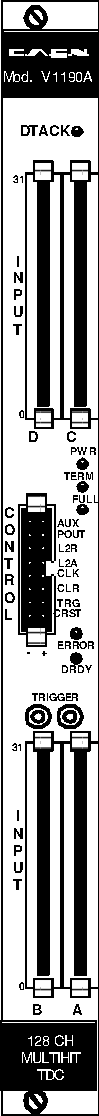
\includegraphics[height = 12cm]{fig/app1/V1190A-front.pdf}
			\caption{\label{fig:DAQSetup:A}}
		\end{subfigure}
		\begin{subfigure}{0.5\linewidth}
		    \centering
			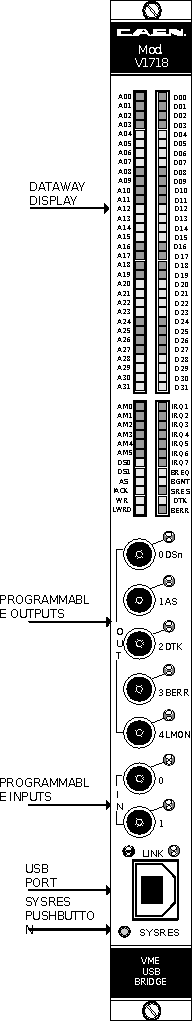
\includegraphics[height = 12cm]{fig/app1/V1718-front.pdf}\\
			\caption{\label{fig:DAQSetup:B}}
		\end{subfigure}
		\begin{subfigure}{\linewidth}
		    \centering
			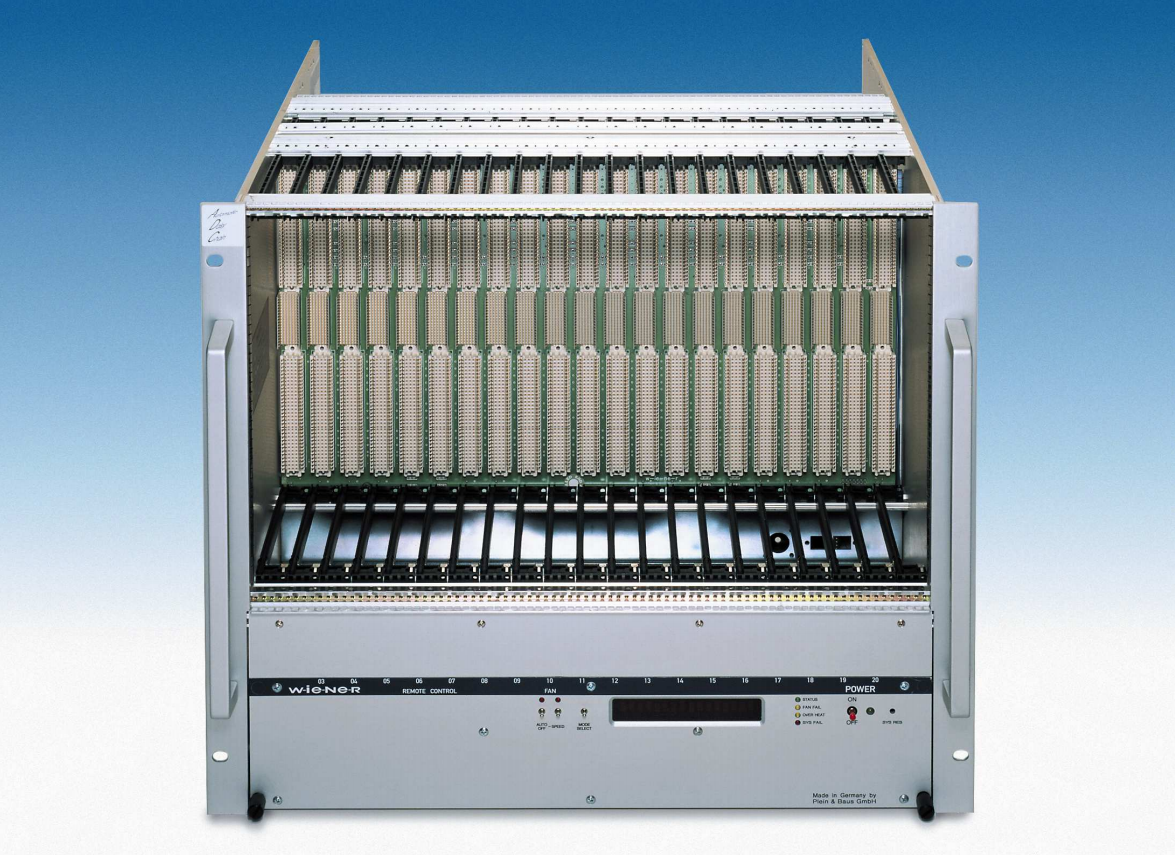
\includegraphics[width = 0.8\plotwidth]{fig/app1/Wiener-front.png}
			\caption{\label{fig:DAQSetup:C}}
		\end{subfigure}
		\caption{\label{fig:DAQSetup} (\ref{fig:DAQSetup:A}) View of the front panel of a V1190A TDC module~\cite{V1190AMUT}. (\ref{fig:DAQSetup:B}) View of the front panel of a V1718 Bridge module~\cite{V1718MUT}. (\ref{fig:DAQSetup:C}) View of the front panel of a 6U 6021 VME crate~\cite{6U6000MUT}.}
	\end{figure}
	
	

\section{Data read-out}
\label{app1:sec:Data}

	To efficiently perform a data readout algorithm, C++ objects to handle the VME modules (TDCs and VME bridge) have been created along with objects to store data and read the configuration file that comes as an input of the DAQ software.\\
	It is useful to remind that the DAQ software in GIF++ is not a standalone software but is called through a \acf{webDCS} application, that is the core of interactions with GIF++ setup, when data needs to be taken. Nevertheless, it is straight forward to make it into a standalone program that could be adapted to any VME setup using V1190A and V1718 modules.\\

    \subsection{V1190A TDCs}
    \label{app1:ssec:V1190A}

	The DAQ used at GIF takes profit of the \textit{Trigger Matching Mode} offered by V1190A modules. This setting is enabled through the method \cppinline{v1190a::SetTrigMatching (int ntdcs)} where \cppinline{ntdcs} is the total number of TDCs in the setup this setting needs to be enabled for (Source Code~\ref{cpp:v1190a}). A trigger matching is performed in between a trigger time tag, a trigger signal sent into the TRIGGER input of the TDC visible on Figure~\ref{fig:DAQSetup:A}, and the channel time measurements, signals recorded from the detectors under test in our case. Control over this data acquisition mode, explained through Figure~\ref{fig:V1190A-TMM}, is offered via 4 programmable parameters:
        
	\begin{itemize}
		\item \textbf{match window:} the matching between a trigger and a hit is done within a programmable time window. This is set via the method\\ \cppinline{void v1190a::SetTrigWindowWidth(Uint windowWidth,int ntdcs)}
		\item \textbf{window offset:} temporal distance between the trigger tag and the start of the trigger matching window. This is set via the method\\ \cppinline{void v1190a::SetTrigWindowWidth(Uint windowWidth,int ntdcs)}
		\item \textbf{extra search margin:} an extended time window is used to ensure that all matching hits are found. This is set via the method\\ \cppinline{void v1190a::SetTrigSearchMargin(Uint searchMargin,int ntdcs)}
		\item \textbf{reject margin:} older hits are automatically rejected to preven buffer overflows and to speed up the search time. This is set via the method\\ \cppinline{void v1190a::SetTrigRejectionMargin(Uint rejectMargin,int ntdcs)}
	\end{itemize}
    
    \begin{figure}[H]
		\centering
		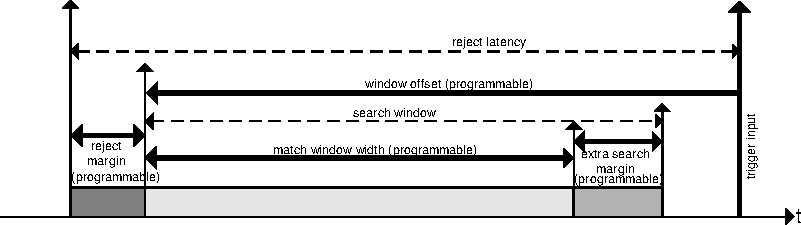
\includegraphics[width = 1.25\plotwidth]{fig/app1/V1190A-TMM.pdf}\\
		\caption{\label{fig:V1190A-TMM} Module V1190A \textit{Trigger Matching Mode} timing diagram~\cite{V1190AMUT}.}
	\end{figure}
	
	Each of these 4 parameters are given in number of clocks, \SI{1}{clock} being \SI{25}{ns} long. It is easy to understand at this level that there are 3 possible functionning settings:
        
	\begin{itemize}
		\item \textbf{1:} the match window is entirely contained after the trigger signal,
		\item \textbf{2:} the match window overlaps the trigger signal, or
		\item \textbf{3:} the match window is entirely contained before the trigger signal as displayed on Figure~\ref{fig:V1190A-TMM}.
	\end{itemize}
	
	In both the first and second cases, the sum of the window width and of the offset can be set to a maximum of \SI{40}{clocks}, which corresponds to \SI{1}{\micro s}. Evidently, the offset can be negative, allowing for a longer match window, with the constraint of having the window ending at most \SI{1}{\micro s} after the trigger signal. In the third case, the maximum negative offset allowed is of \SI{2048}{clocks} (12 bit) corresponding to \SI{51.2}{\micro s}, the match window being strictly smaller than the offset. In the case of GIF++, the choice has been made to use this last setting by delaying the trigger signal. During the studies performed in GIF++, both the efficiency of the RPCs, probed using a muon beam, and the noise or gamma background rate are monitored. The extra search and reject margins are left unused.\\
	To probe the efficiency of RPC detectors, the trigger time tag is provided by the coïncidence of scintillators when a bunch of muons passes through GIF++ area is used to trigger the data acquisition. For this measurement, it is useful to reduce the match window width only to contain the muon information. Indeed, the delay in between a trigger signal and the detection of the corresponding muon in the RPC being very contant (typically a few tens of ns due to jitter and cable length), the muon signals are very localised in time. Thus, due to a delay of approximalety \SI{325}{ns} in between the muons and the trigger, the settings where chosen to have a window width of \SI{24}{clocks} (\SI{600}{ns}) centered on the muon peak thanks to a negative offset of \SI{29}{clocks} (\SI{725}{ns}).\\
	On the otherhand, monitoring the rates don't require for the DAQ to look at a specific time window. It is important to integrate enough time to have a robust measurement of the rate as the number of hits per time unit. The triggerring signal is provided by a pulse generator at a frequency of \SI{300}{Hz} to ensure that the data taking occurs in a random way, with respect to beam physics, to probe only the irradiation spectrum on the detectors. The match window is set to \SI{400}{clocks} (\SI{10}{\micro s}) and the negative offset to \SI{401}{clocks} as it needs to exceed the value of the match window.\\
	
	\begin{code}
	\captionof{listing}{Description of C++ object v1190a}
	\label{cpp:v1190a}
	
    \begin{cppcode}
class v1190a
{
 private :
    long              Handle;
    vector<Data32>    Address;
    CVDataWidth       DataWidth;
    CVAddressModifier AddressModifier;

 public:

    v1190a(long handle, IniFile *inifile, int ntdcs);
    ~v1190a();
    Data16 write_op_reg(Data32 address, int code, string error);
    Data16 read_op_reg(Data32 address, string error);
    void   Reset(int ntdcs);
    void   Clear(int ntdcs);
    void   TestWR(Data16 value,int ntdcs);
    void   CheckTDCStatus(int ntdcs);
    void   CheckCommunication(int ntdcs);
    void   SetTDCTestMode(Data16 mode,int ntdcs);
    void   SetTrigMatching(int ntdcs);
    void   SetTrigTimeSubstraction(Data16 mode,int ntdcs);
    void   SetTrigWindowWidth(Uint windowWidth,int ntdcs);
    void   SetTrigWindowOffset(Uint windowOffset,int ntdcs);
    void   SetTrigSearchMargin(Uint searchMargin,int ntdcs);
    void   SetTrigRejectionMargin(Uint rejectMargin,int ntdcs);
    void   GetTrigConfiguration(int ntdcs);
    void   SetTrigConfiguration(IniFile *inifile,int ntdcs);
    void   SetTDCDetectionMode(Data16 mode,int ntdcs);
    void   SetTDCResolution(Data16 lsb,int ntdcs);
    void   SetTDCDeadTime(Data16 time,int ntdcs);
    void   SetTDCHeadTrailer(Data16 mode,int ntdcs);
    void   SetTDCEventSize(Data16 size,int ntdcs);
    void   SwitchChannels(IniFile *inifile,int ntdcs);
    void   SetIRQ(Data32 level, Data32 count,int ntdcs);
    void   SetBlockTransferMode(Data16 mode,int ntdcs);
    void   Set(IniFile *inifile,int ntdcs);
    void   CheckStatus(CVErrorCodes status) const;
    int    ReadBlockD32(Uint tdc, const Data16 address,
               Data32 *data, const Uint words, bool ignore_berr);
    Uint   Read(RAWData *DataList,int ntdcs);
};
    \end{cppcode}
    \end{code}
	
	The v1190a object, defined in the DAQ software as in Source Code~\ref{cpp:v1190a}, offers the possility to concatenate all TDCs in the readout setup into a single object containing a list of hardware addresses (addresses to access the TDCs' buffer through the VME crate) and each constructor and method acts on the list of TDCs.\\
	
	\subsection{DataReader}
	\label{app1:ssec:DataReader}
	
	Enabled thanks to \cppinline{v1190a::SetBlockTransferMode(Data16 mode, int ntdcs)}, the data transfer is done via \acf{BLT}. Using BLT allows to tranfer a fixed number of events called a \textit{block}. This is used together with an \acf{AFL} of the TDCs' output buffers, defined through \cppinline{v1190a::SetIRQ(Data32 level, Data32 count,int ntdcs)}. This AFL gives the maximum amount of 32 bits words that can writen in the buffer before an \acf{IRQ} is generated and seen by the VME Bridge, stopping the data acquisition to transfer the content of each TDC buffers before resuming. The AFL can, at maximum, be of 32735 words (16 bits). This number corresponds to the depth of the output buffer of a TDC. For each trigger, 6 words or more are written into the TDC buffer:
	
	\begin{itemize}
		\item \textbf{a global header} providing information of the event number since the beginning of the data acquisition,
		\item \textbf{a TDC header},
		\item \textbf{the TDC data} (if any), 1 for each hit recorded during the event, providing the channel and the time stamp associated to the hit,
		\item \textbf{a TDC error} providing error flags,
		\item \textbf{a TDC trailer},
		\item \textbf{a global trigger time tag} that provides the absolute trigger time relatively to the last reset, and
		\item \textbf{a global trailer} providing the total word count in the event.
	\end{itemize}
	
	As previously described in Section~\ref{ssec:PulseProc}, CMS RPC FEEs provide us with \SI{100}{ns} long LVDS output signals that are injected into the TDCs' input. Any avalanche signal that gives a signal above the FEEs threshold is thus recorded by the TDCs as a hit within the match window. Each hit is assigned to a specific TDC channel with a time stamp with a precision of \SI{100}{ps}. The reference time, the 0, is provided by the beginning of the match window. Thus for each trigger, coming from a scintillator coïncidence or the pulse generator, a list of hits is stored into the TDCs buffers and will then be transfered into a ROOT Tree.\\
	
	When the BLT is used, it is easy to understand that the maximum number of words that have been set as ALF will not be a finite number of events or, at least, the number of events that would be recorded into the TDC buffers will not be a multiple of the block size. In the last BLT cycle to tranfer data, the number of events to transfer will most propably be lower than the block size. In that case, the TDC can add fillers at the end of the block but this option requires to send more data to the computer and is thus a little slower. Another solution is to finish the transfer after the last event by sending a bus error that states that the BLT reached the last event in the pile. This method has been chosen in GIF++.\\
	
	Due to irradiation, an event in GIF++ can count up to 300 words per TDC. A limit of 4096 words (12 bits) has been set to generate IRQ which represent from 14 to almost 700 events depending on the average of hits collected per event. Then the block size has been set to 100 events with enabled bus errors. When an AFL is reached for one of the TDCs, the VME bridge stops the acquisition at the hardware level by sending a NIM pulse out of one of the 5 programmable outputs to the VETO of the coíndidence module where the trigger signals originate from. As long as this signal is ON, no trigger reaches the TDCs anymore.\\
	
	The data is then transfered one TDC at a time into a structure called \cppinline{RAWData} described below.\\
	
	\begin{cppcode}
struct RAWData{
    vector<int>            *EventList;
    vector<int>            *NHitsList;
    vector<int>            *QFlagList;
    vector<vector<int> >   *ChannelList;
    vector<vector<float> > *TimeStampList;
};
    \end{cppcode}
    
	In order to organize the data transfer and the data storage, an object called \cppinline{DataReader} was created. On one hand, it has members of the \cppinline{v1718} and \cppinline{v1190a} classes for communication purposes, such as VME modules settings via a configuration file \cppinline{IniFile *iniFile} or data read-out through \cppinline{v1190a::Read()} and on the other hand, it contains the struture \cppinline{RAWData} that allows to organise the data in vectors reproducing the tree structre of a ROOT file.\\
	
	\begin{cppcode}
class DataReader
{
    private:
        bool     StopFlag;
        IniFile *iniFile;
        Data32   MaxTriggers;
        v1718   *VME;
        int      nTDCs;
        v1190a  *TDCs;
        RAWData  TDCData;

    public:
        DataReader();
        virtual ~DataReader();
        void     SetIniFile(string inifilename);
        void     SetMaxTriggers();
        Data32   GetMaxTriggers();
        void     SetVME();
        void     SetTDC();
        int      GetQFlag(Uint it);
        void     Init(string inifilename);
        void     FlushBuffer();
        void     Update();
        string   GetFileName();
        void     WriteRunRegistry(string filename);
        void     Run();
};
    \end{cppcode}
    
    Each event is saved into \cppinline{TBranch} of a ROOT \cppinline{TTree} as 3 integers that represent the event ID (\cppinline{EventCount}), the number of hits read from the TDCs (\cppinline{nHits}), the quality flag that provides information for any problem in the data transfer (\cppinline{qflag}), and 2 lists of nHits elements containing the fired TDC channel (\cppinline{TDCCh}) and their respective time stamps (\cppinline{TDCTS}).\\
    
    \begin{cppcode}
RAWData TDCData;
TFile *outputFile = new TFile(outputFileName.c_str(),"recreate");
TTree *RAWDataTree = new TTree("RAWData","RAWData");

int           EventCount = -9;
int           nHits = -8;
int           qflag = -7;
vector<int>   TDCCh;
vector<float> TDCTS;

RAWDataTree->Branch("EventNumber",&EventCount, "EventNumber/I");
RAWDataTree->Branch("number_of_hits",&nHits,"number_of_hits/I");
RAWDataTree->Branch("Quality_flag",&qflag,"Quality_flag/I");
RAWDataTree->Branch("TDC_channel",&TDCCh);
RAWDataTree->Branch("TDC_TimeStamp",&TDCTS);

//...
//Here read the TDC data and place it into TDCData for as long
//as you didn't collect the requested amount of data.
//...
    
for(Uint i=0; i<TDCData.EventList->size(); i++){
    EventCount  = TDCData.EventList->at(i);
    nHits       = TDCData.NHitsList->at(i);
    qflag       = TDCData.QFlagList->at(i);
    TDCCh       = TDCData.ChannelList->at(i);
    TDCTS       = TDCData.TimeStampList->at(i);
    RAWDataTree->Fill();
}
    \end{cppcode}

    \subsection{V1718 USB Bridge}
    \label{app1:ssec:V1718}
    
    Previously, we discussed the data transfer using a combination
	
	The v1718 object is defined in the DAQ software as followed.\\
	
	\begin{cppcode}
class v1718{

    private :
        int               Handle;

        Data32            Data;           // Data
        CVIRQLevels       Level;          // Interrupt level
        CVAddressModifier AM;             // Addressing Mode
        CVDataWidth 	  DataSize;       // Data Format
        Data32            BaseAddress;    // Base Address

    public:
        v1718(IniFile *inifile);
        ~v1718();
        long              GetHandle(void) const;
        int               SetData(Data16 data);
        Data16            GetData(void);
        int               SetLevel(CVIRQLevels level);
        CVIRQLevels       GetLevel(void);
        int               SetAM(CVAddressModifier am);
        CVAddressModifier GetAM(void);
        int               SetDatasize(CVDataWidth datasize);
        CVDataWidth       GetDataSize(void);
        int               SetBaseAddress(Data16 baseaddress);
        Data16            GetBaseAddress(void);
        void              CheckStatus(CVErrorCodes status) const;
        bool              CheckIRQ();
        void              SetPulsers();
        void              SendBUSY(BusyLevel level);
};
    \end{cppcode}
    
    \subsection{DAQ algorithm overview}
    \label{app1:ssec:algo}
    
    

\section{Software export}


\clearpage{\pagestyle{empty}\cleardoublepage}
